\section{Mathematische Grundlagen}

\textbf{Kinematik} ist die reine geometrische Beschreibung von Bewegung eines Manipulators
oder Roboters. Das essentielle Konzept ist die \textbf{Position}.

\textbf{Statik} behandelt Kräfte und Momente, die sich auf einen ruhenden Mechanismus
auswirken. Das essentielle Konzept ist die \textbf{Steifigkeit}.

\textbf{Dynamik} analysiert die Kräfte und Momente, die durch Bewegung und Beschleunigung
eines Mechanismus und einer zusätzlichen Last entstehen.

\textbf{Terminologie}:
\begin{center}
	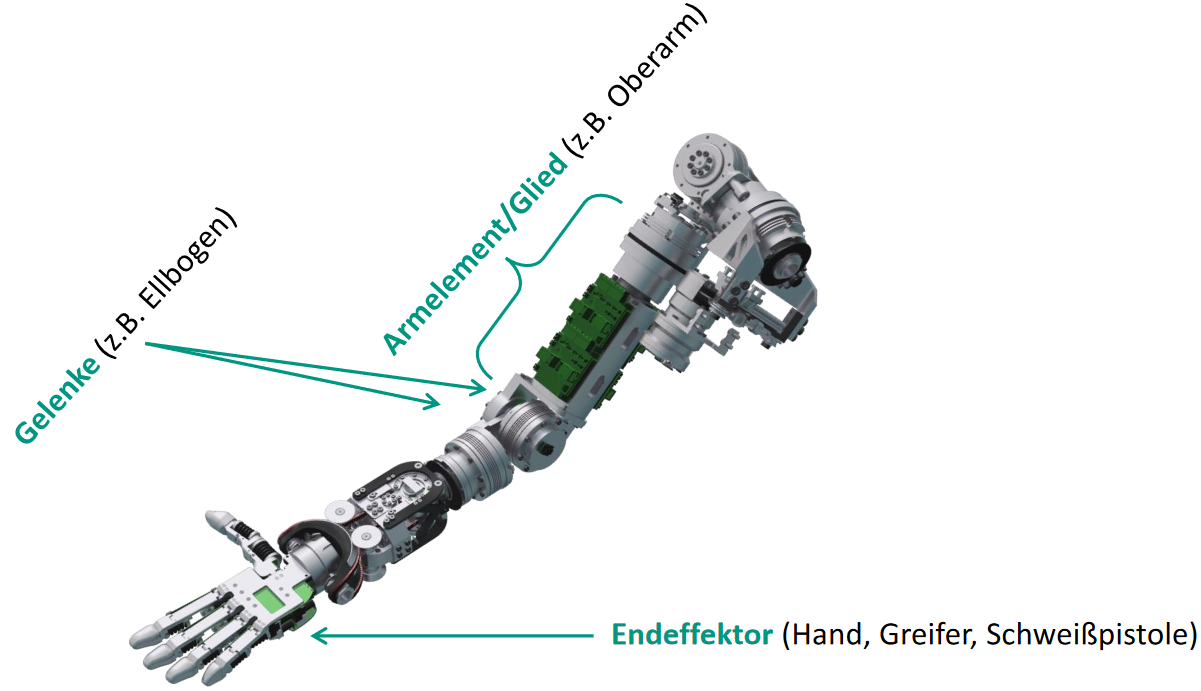
\includegraphics[width=0.7\textwidth]{images/arm.png}
\end{center}
\medskip
\textbf{Kinematische Kette} ist eine Menge an Gliedern, die durch Gelenke verbunden sind.

\textbf{Freiheitsgrade} (DoF) ist die Anzahl unabhängiger Parameter, die zur kompletten Spezifikation der Lage eines Objekts benötigt werden, z.B. Starrkörper hat in 2D 3 DoF und in 3D 6 DoF.

\textbf{Starrkörperbewegungen werden durch zwei Eigenschaften charakterisiert}:
\begin{enumerate}
	\item Distanz zweier beliebiger Punkte ist konstant
	\item Orientierungen im Körper bleiben erhalten
\end{enumerate}

\textbf{SO(3) und SE(3)}:
\begin{itemize}
	\item SO(3): \textbf{Spezielle Orthogonale Gruppe}, die \textbf{Rotationen} repräsentiert
	\item SE(3): \textbf{Spezielle Euklidische Gruppe}, die \textbf{Transformationen} repräsentiert
	\item Elemente aus SO(3) werden als reale $3\times3$ orthogonale Matrizen $R$ (Zeilen- und Spaltenvektoren orthonormal) beschrieben und erfüllen
	$$R^\top R=1 \qquad \text{ mit } \qquad\det(R)=1$$
	\item Elemente aus SE(3) sind von der Form $(\mathbf{p},R)$ mit $\mathbf{p}\in\R^3$ und $R\in\text{SO(3)}$ und beschreiben Verknüpfungen von Rotationen und Translationen
	\begin{center}
		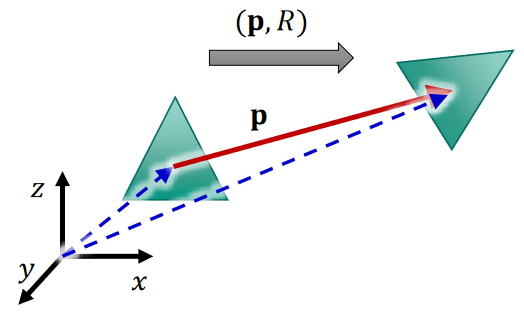
\includegraphics[width=0.4\textwidth]{images/se3.png}
	\end{center}
\end{itemize}
\medskip
\textbf{Euklidischer Raum}: Vektorraum $\R^3$ mit dem Skalarprodukt.
\begin{itemize}
	\item Punkt $\mathbf{a}$ im euklidischen Raum wird durch Vielfache der Einheitsvektoren $\mathbf{e_x}, \mathbf{e_y}, \mathbf{e_z}$ beschrieben
	\item Wir benutzen \textbf{rechtsdrehende Koordinatensysteme}
\end{itemize}
\begin{center}
	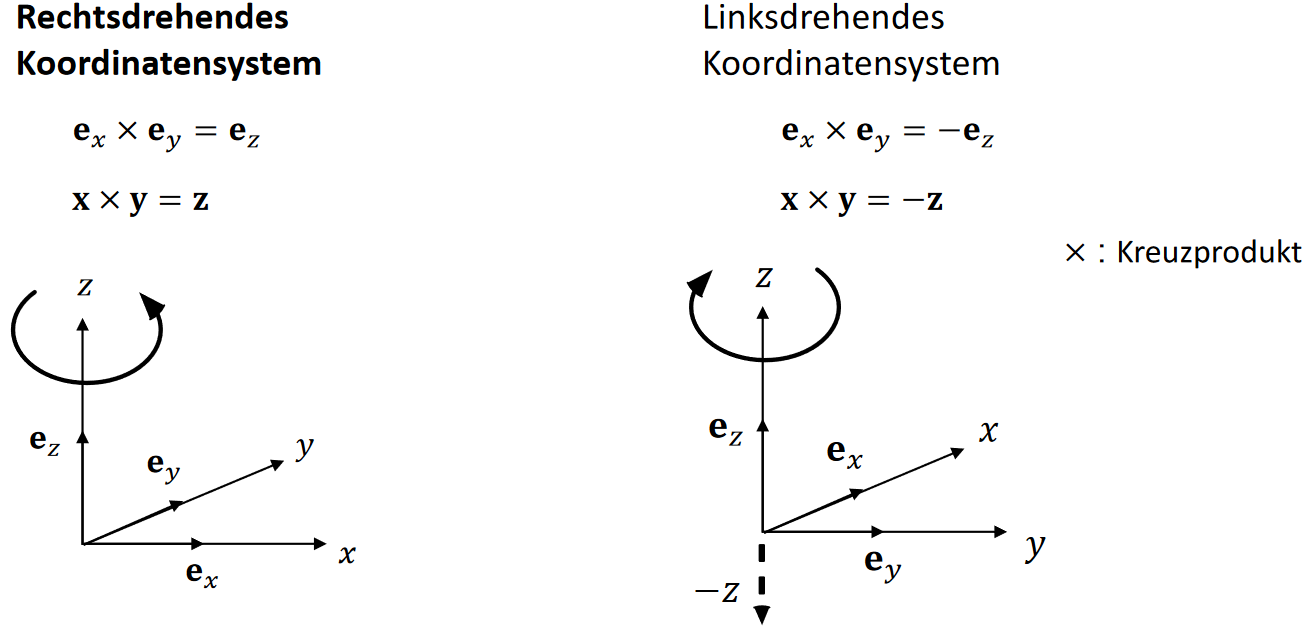
\includegraphics[width=0.75\textwidth]{images/koordinaten.png}
\end{center}
\medskip
\textbf{Lineare Abbildungen}  (Transformationen), die den euklidischen Raum auf sich selbst abbilden, nennt man \textbf{Endomorphismen}: $$\phi(\cdot)\colon\R^3\rightarrow\R^3$$
\begin{itemize}
	\item Endomorphismen können durch quadratische Matrizen repräsentiert werden: $$\phi(\mathbf{a})=A\cdot\mathbf{a},\qquad A\in R^{3\times 3}$$
	\item $A$ beschreibt einen Basiswechsel zwischen den originalen Basisvektoren $\mathbf{e_x}, \mathbf{e_y}, \mathbf{e_z}$ und den neuen Basisvektoren $\mathbf{e_x'}, \mathbf{e_y'}, \mathbf{e_z'}$:
	
	$$A=\irow{\mathbf{e_x'}&\mathbf{e_y'}&\mathbf{e_z'}}\cdot\irow{\mathbf{e_x}&\mathbf{e_y}&\mathbf{e_z}}^{-1}$$
\end{itemize}
\pagebreak

\textbf{Bijektive} Endomorphismen nennt man \textbf{Isomorphismen}.
\begin{itemize}
	\item Eigenschaften:
	\begin{enumerate}
		\item Winkel bleiben erhalten
		\item Längen bleiben erhalten
		\item Händigkeit beleibt erhalten
	\end{enumerate}
	\item Eine spezielle Art von Isomorphismen ist die \textbf{Rotationsgruppe} SO(3)
\end{itemize}
\medskip
\textbf{Rotationsgruppe SO(3):}
\begin{itemize}
	\item SO(3) ist nicht kommutativ: $A\cdot B\cdot \mathbf{x}\neq B\cdot A\cdot \mathbf{x}$ mit $\mathbf{x}\in\R^3$ und $A,B\in\text{SO(3)}$ 
	\item Für alle $R\in\text{SO(3)}$ ist $R^{-1}=R^\top$, die Inverse kann also leicht berechnet werden
\end{itemize}
\medskip
\textbf{Rotationen in 2D}:
\begin{itemize}
	\item Rotation in der $xy$-Ebene um $(0,0)$ ist eine \textbf{lineare Transformation}
	\item \textbf{Rotationsmatrix}: $R_\alpha(\mathbf{x})=
	\left(\begin{matrix}
		\cos\alpha & -\sin\alpha \\
		\sin\alpha & \cos\alpha 
	\end{matrix}\right)\cdot\mathbf{x}$
	mit $RR^\top=R^\top R=I$ und $\det(R)=1$
	\item Rotation um einen Punkt $\mathbf{c}\neq(0,0)$ ist keine lineare Transformation.
	Verschiebe dafür die Ebene um $-\mathbf{c}$, rotiere und verschiebe wieder um $+\mathbf{c}$ zurück:
	$$R_{\mathbf{c},\alpha}=R_\alpha(\mathbf{x}-\mathbf{c})+\mathbf{c}= R_\alpha(\mathbf{x})+(-R_\alpha(\mathbf{c})+\mathbf{c})$$
	\item $R_{\mathbf{c},\alpha}$ ist eine nichtlineare Transformation und heißt \textbf{affine Transformation}.
	Sie unterscheidet sich von $R_\alpha$ nur durch das Addieren einer Konstante
\end{itemize}
\medskip
\textbf{Rotationen in 3D}:
\begin{itemize}
	\item Eine 2D Rotation in der $xy$-Ebene ist eine 3D Rotation um die $z$-Achse: $$R_{\mathbf{z},\alpha}=\left(\begin{matrix}
		\cos\alpha & -\sin\alpha & 0 \\
		\sin\alpha & \cos\alpha & 0 \\
		0 & 0 & 1
	\end{matrix}\right)$$
	\item Rotationen können verkettet werden: $\phi_{\mathbf{z},\gamma}\left(\phi_{\mathbf{y},\beta}\left(\phi_{\mathbf{x},\alpha}(\mathbf{a})\right)\right),\qquad \mathbf{a}\in\R^3$
\end{itemize}
\medskip
\textbf{Probleme mit Rotationsmatrizen}:
\begin{itemize}
	\item \textbf{Redundanz}: Neun Werte für eine Rotationsmatrix
	\item Probleme im Bereich des maschinellen Lernens
\end{itemize}
\pagebreak

\textbf{Eulerwinkel}:
\begin{itemize}
	\item Es ist möglich jede Rotation durch drei Rotationen um jeweils eine Rotationsachse darzustellen
	\item \textbf{Euler-Konvention}: $\mathbf{z}\text{ }\mathbf{x'}\text{ }\mathbf{z''}$ (lokale Drehung, Drehung verändert Achsen) oder $\mathbf{x}\text{ }\mathbf{y}\text{ }\mathbf{z}$ (globale Drehung, Drehung um feste Achsen)
	\item Winkel $\alpha,\beta,\gamma$ sind \textbf{Eulerwinkel} und beschreiben den Grad der Drehungen
	\begin{center}
		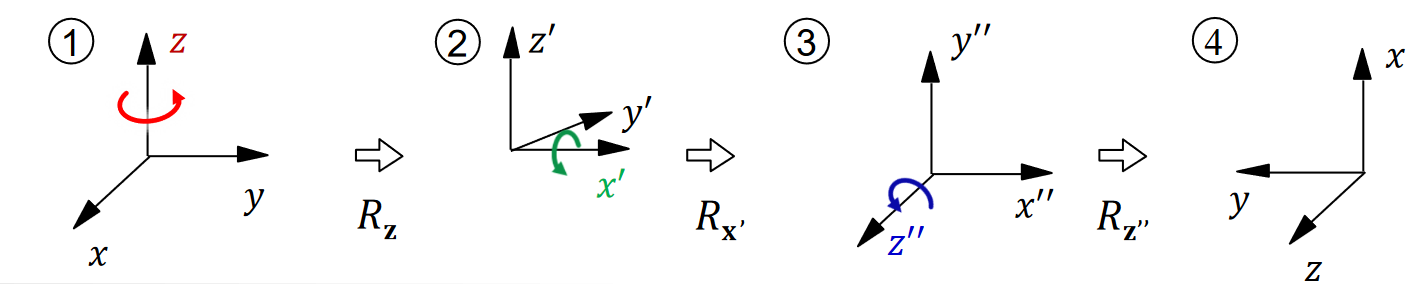
\includegraphics[width=0.7\textwidth]{images/euler.png}
	\end{center}
	\item \textbf{Vorteile}: Kompakter und aussagekräftiger als Rotationsmatrizen
	\item \textbf{Nachteil}: 
	\begin{itemize}
		\item Nicht eindeutig: In der Euler-Konvention $\mathbf{x}\text{ }\mathbf{y'}\text{ }\mathbf{z''}$ beschreiben die Eulerwinkel $(45^\circ,-90^\circ,45^\circ)$ und 
		und $(30^\circ,-90^\circ,60^\circ)$ die gleiche Rotation
		\item Nicht kontinuierlich: Kleine Änderung in der Orientierung können zu großen Änderungen der Eulerwinkel führen
		\item \textbf{Gimbal Lock}: Bei bestimmten Winkeln werden zwei Achsen voneinander abhängig $\Rightarrow$ Ein Freiheitsgrad geht verloren
	\end{itemize}
\end{itemize}
